\chapter{Design}

% The design should describe what you expected to do, and might also explain areas that you had to revise after some investigation.

% Typically, for an object-oriented design, the discussion will focus on the choice of objects and classes and the allocation of methods to classes. The use made of reusable components should be described and their source referenced. Particularly important decisions concerning data structures usually affect the architecture of a system and so should be described here.

% How much material you include on detailed design and implementation will depend very much on the nature of the project. It should not be padded out. Think about the significant aspects of your system. For example, describe the design of the user interface if it is a critical aspect of your system, or provide detail about methods and data structures that are not trivial. Do not spend time on long lists of trivial items and repetitive descriptions. If in doubt about what is appropriate, speak to your supervisor.

% You should concentrate on the more important aspects of the design. It is essential that an overview is presented before going into detail. As well as describing the design adopted it must also explain what other designs were considered and why they were rejected.

\section{Introduction}
The technical design of an application is, in essence, the intersection of current ``best practice'' in the software development field (and the related programming language communities), its target domains and the user needs.

``Technically'', FundFind:
\begin{itemize}
 \item is a web application
 \item is written in Python
 \item stores its data in an asynchronous NoSQL data store with built-in search capabilities
 \item has a mobile-friendly web interface
 \item exposes all its major features via an API
\end{itemize}

These characteristics have not changed since the start of the project. The technical decisions that stand behind them proved to be mostly correct and helpful, and are elaborated upon in the next section.

\subsection{Design Details and Rationale}
\label{design-rationale}

FundFind
\begin{itemize}
 \item is a web application
 
This was decided right from the start of the project. The way current Open Knowledge Foundation and Cottage Labs projects worked was important since one of the two major target domains is Open Data / Knowledge and Cottage Labs is an interested party. Most OKFN projects are web applications - even the library ones have mostly been used in web applications. Cottage Labs have also focussed on web applications. Such applications have just proven themselves to be far more ``co-operative'' than traditional desktop applications - easy to access, easy to modify so that they expose their data via an API (interoperability). \S\ref{api-tech-design} details further interoperability decisions - the transport format (JSON) and protocol (HTTP).
 
 \item is written in Python

Similar factors to the interoperability point raised above played a role in deciding the language of the application. A lot of Open Knowledge projects use Python \cite{nomenklatura, offenesparlament, pybossa, activityapi} - the same goes for Cottage Labs projects \cite{leaps, portality, iioa, artemis, cl-web-code, xcri, negotiator}. The language is also simple and strives encourage and enable readability - ``code is read much more often than it is written'' \cite{pep8}.
 
 \item stores its data in an asynchronous NoSQL data store with built-in search capabilities
 
 FundFind relies on elasticsearch to store its data. Elasticsearch is an indexing server which allows for sophisticated search queries against a body of text and other data \cite{es}. The essential advantages were simplicity, performance, usage by other Cottage Labs projects and certain options it leaves open for further development (see \S\ref{design-datastore}).
 
 \item has a mobile-friendly web interface
 
 FundFind is an application which tries to enable sharing of information - one of the highest priority features. Owing to the nature of the information it makes sense to try to make it mobile-friendly - scholars do not necessarily have to hear about funding opportunities while sitting at their desks.
 
 Whether they will also want to share this rather dense information while on the go is another matter entirely. Mobile-friendliness was not noted as having particularly high priority in the Progress Report, and it still does not - it was just easy to implement due to the fact that the libraries used to make the web user interface follow current best software engineering practice. More details are available in \S\ref{impl-ui}. Essentially, making a good UI by using the libraries properly would have led to a mobile-friendly UI (at the flick of a filename and a few CSS class names).
 
 \item exposes all its major features via an API
 
 The JISC Report ``Advantages of APIs'' states ``the API enables use and re-use; it is a tool by which we can disseminate knowledge'' \cite{advantages-apis}. This is the essential advantage of API-s and the reason the concept of an API has become one of the building blocks of the Open Knowledge movement. If FundFind aims to prototype a useful tool which will eventually contribute to Open Data (so taking into account the needs of the ``analytical'' audience group from \S\ref{audience-analyse}), it needs to eventually have an API. It is simply better to design the project with the API in mind instead of tacking it on later. One example is the HiFi project, which had the following to say on the subject:
 
 \begin{shadequote}
  We built the API to satisfy these requirements first, then we built our app on top of the API. This turned out to be a great idea. We got to dogfood our API for the entire development process and it made testing a lot simpler.
  \par\emph{Kris Jordan in ``First we built an API, then we built a CMS'' \cite{hifi-api}}
 \end{shadequote}
 
\end{itemize}

\section{Overall Architecture}
% diagram of architecture
% changes from progress report - any?, why? why not?
% these are all MODULES, not CLASSES - explain difference, rationale for using (convention at least)

\begin{figure}[H]
\centering
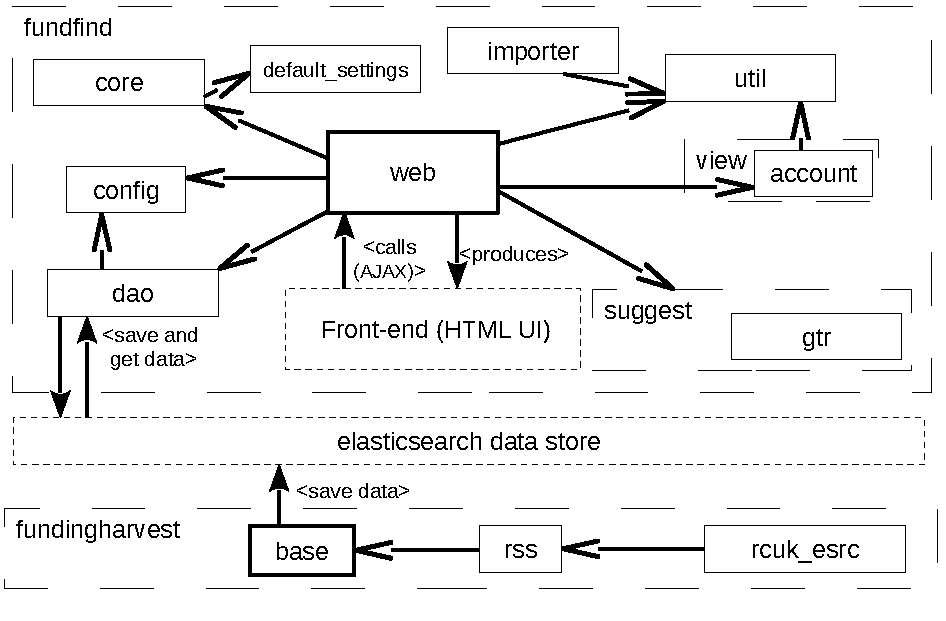
\includegraphics[width=1.00\textwidth,]{Chapter3/overview_design.pdf}
\caption{Overview of FundFind and Funding Harvest's technical architecture.}
\label{fig:arch}
\end{figure}

The entities drawn with continuous lines in the diagram are modules - collections of code related to solving the same problem. The contents of the modules - the details of the technical design of the main application - are discussed below in \S\ref{design-main-first} to \S\ref{design-main-last}.

The entities drawn with a heavy continuous line are the entry points - they are the modules which actually (need to) get run by the Python interpreter.

The entities drawn with a rough dashed line are packages. Packages and modules are simply ways of organising code in Python and are discussed in more detail below.

The entities drawn with a fine dashed line are more abstract concepts (datastore and user interface) which are elaborated upon below.

Full listing of all source code files with notes is available in ``\titleref{file-listings}'', Appendix \ref{file-listings}.

\subsection{Organising code in Python}
Traditionally Object-Oriented Programming talks about ``classes'' as, essentially, blueprints combining data structures and imperative code (methods) together. These can then be ``instantiated'' to produce a concrete ``object''.

This is of course well-supported in Python. However, Python also has an additional convention when it comes to organising code - ``modules''. The Python documentation says ``You may also want to use a handy function that you’ve written in several programs without copying its definition into each program.'' \cite{python-doc-modules}. While re-use of code is usually achieved by making everything an object in other languages like Java, Python actually allows functions and even just code statements at the top level of a source code file. Thus, instead of having to create a ``Util'' class with several static methods, Python authors are encouraged to simply define the functions they need at the module level. In other words, modules are a convenient way to bundle together \emph{related} pieces of code - whether that would just be a sequence of statements, function or class definitions. This may seem messy but has proven to be quite efficient by essentially allowing the developer to better express their mental model 
of how their program should be organised, instead of forcing a particular structure.

An obvious characteristic of Python modules is that they are also implicit namespaces. Thus, the built-in |int()| can easily be distinguished from |random.int()|. A Python program would have to |import random| before it can use |random.int()|.

In this case, |random| happens to be a module that is part of the standard Python distribution. However, exactly the same rules apply to user-defined modules. Thus, the dotted arrows which connect the modules in Figure \ref{fig:arch} essentially mean ``module X imports module Y and uses something from Y''.

Packages are simply a collection of modules. Since a module is a file, packages are just directories (containing a possibly empty |__init__.py| file) - another way to organise related code.

To sum up, packages contain modules. Modules could contain classes (alongside any other code and function definitions).

% TODO Furthermore, certain naming conventions exist in Python for package, module and class names.

\subsection{Changes over time}
% TODO redo this with a diagram showing the real initial IDFind code and showing deleted modules in red, added modules in green
The modules which form the main web application have not changed much from the parent IDFind project. An overview of IDFind's technical design presented in the Progress Report \cite{progress-report} had actually left out the |util| module and mistakenly used the term ``class'' to refer to certain modules.

% TODO delete this bullshit after creating diagram in prev. TODO
This diagram is reproduced in Figure \ref{fig:idfind-uml}. Since it was supposed to be a rough overview, another IDFind module was left out - the |tweetlisten| module allows IDFind to respond to Twitter requests in a similar fashion as if the user was using the web user interface. This module was scrapped in FundFind since potential target users (including the author) just could not think of a way in which Twitter integration would be immediately useful. On the other hand, writing any sensible test coverage for an external service would have taken up valuable time which was used for more important features.

This raises another important point - usually, tests can be inherited alongside features from parent codebases. However, IDFind had no automated tests, making for the decision to actually scrap the Twitter integration instead of just leaving it in the FundFind codebase due to FundFind's more comprehensive testing strategy. This is elaborated upon in \S\ref{testing-intro}.

% TODO this is unfinished!
In terms of further changes, the Harvesters package was added

Finally, the contents of all of thes

\begin{figure}[H]
\centering
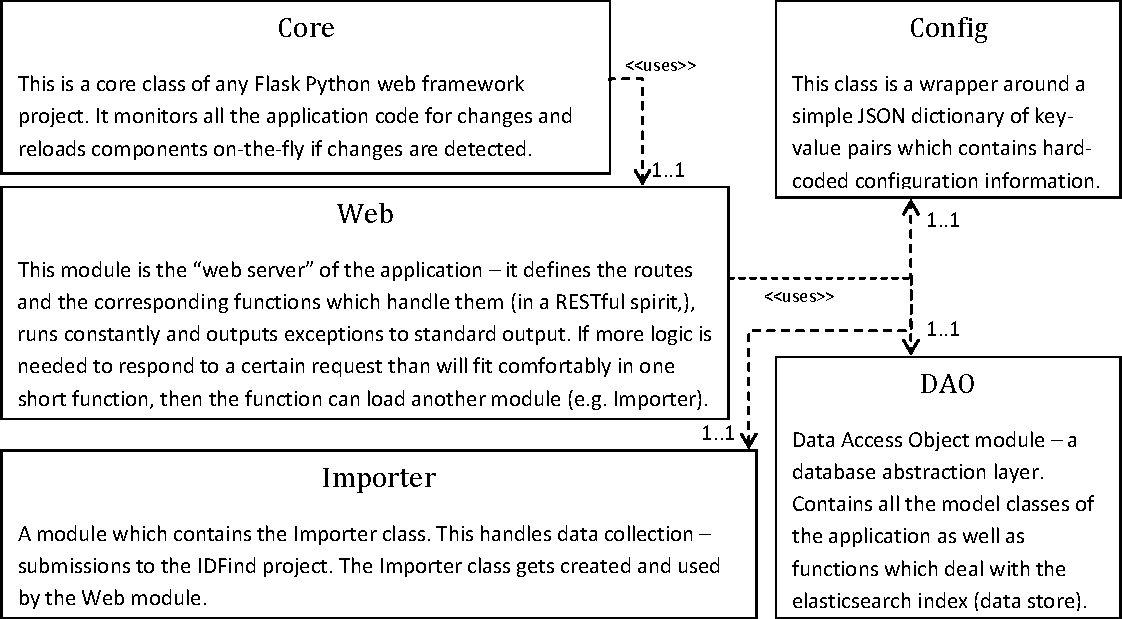
\includegraphics[width=1.00\textwidth,]{Chapter3/idfind-uml.pdf}
\caption{Overview of parent project IDFind's technical design presented in the Progress Report \cite{progress-report}}
\label{fig:idfind-uml}
\end{figure}

Figure \ref{fig:idfind-uml} was intended only as an overview and had intentionally left out

\section{fundfind}
\label{design-main-first}
% TODO remember to include classes contained within these modules in each module's description

\subsection{core}
The Flask Python web framework is used in this project. %TODO what does flask do from site and cite
%TODO point towards chapter 4 relevant section for more details
|core| is, by convention (as many other things in Python) the name of the main module in a Flask-based application. It monitors all application code for changes and (in debug mode) reloads components on-the-fly if changes are detected.

\subsection{DAO}
Data Access Object module – a database abstraction layer. Contains all the model classes of the application as well as functions which deal with the elasticsearch index (data store).

\subsection{Web}
This module is the ``web server'' of the application – it defines the routes and the corresponding functions which handle them (in a RESTful way), runs constantly and outputs exceptions to standard output. If more logic is needed to respond to a certain request than will fit comfortably in one short function, then the function can load another module (e.g. Importer).

\subsection{Importer}
A module which contains the Importer class. This handles data collection – submissions to the IDFind project. The Importer class gets created and used by the Web module.

\subsection{Config}
This class is a wrapper around a simple JSON dictionary of key-value pairs which contains hard-coded configuration information.

\subsubsection{Default Settings}

\subsection{Util}

\section{suggest}

\subsection{gtr}

\section{fundingharvest}
\label{design-main-last}

\subsection{HarvesterBase}


\subsection{RssHarvesterBase}
% TODO explain why a base class with inheritance - used to have CLI submitter as well as an e-mail harvester, but dropped - however design still good and extendable

\subsubsection{EsrcRssHarvester}

\section{Datastore}
\label{design-datastore}
 Indexing software is usually most easily understood in comparison to more traditional approaches of storing data, like relational databases (MySQL \cite{mysql}, Oracle \cite{oracle}). These store data in a highly structured way and the base structural unit is a table (theoretically equivalent to a set, which is where relational theory and such databases come from). The ``indexing'' part actually means ``analysis'' in the broadest sense. Given data - any data, images, text, Microsoft Word binary blobs pretending to be text - the software will try to find common features or look for certain characteristics in the data. For example, it will try to discern whether a particular string actually represent a datetime value.
 
 Elasticsearch is actually a NoSQL datastore - which essentially means that it deals with very simple key-value pairs as the basic unit of organising data \emph{instead of} tables, or sets. It also supports slightly more complex, but still very simple structures, such as lists and dictionaries (a.k.a. HashMaps). This means that the storage representation is also quite simple - in this case, all documents stored within an elasticsearch instance can be represented in the JSON data format. This simplicity enables elasticsearch to deal with semistructured data much more easily than a traditional relational database.
 
 A lot of funding data can be considered semistructured - one type of funding call might have a closing date, another one might not. When multiple data sources are considered it becomes even more difficult since different organisations publish different bits of data about their available funding. Since elasticsearch combines its simple storage with a powerful, fast search engine this makes such ``holes'' in the data a lot less important than usual - the ``usefulness'' of the data scales with its quality (there is no getting around the fact that less holes is better), but \emph{the software can deal with it} without throwing null pointer exceptions and \emph{the data that is present is still easily discoverable}.
 
 % TODO REVIEW include an example of a JSON document that FundFind has, and then represent the same document using a relational structure of several tables. Point out how many are needed and that it's cumbersome. Concede that it gives a speed advantage with a lot of records, but retort that elasticsearch already achieves that speed just by searching the data instead of structuring it in a specific way, so the database can find it more quickly on disk...
 
 Elasticsearch's RESTful JSON-returning API usually enables rapid prototyping, evaluation and integration with Javascript visualisation libraries such as d3 \cite{d3} and BubbleTree \cite{bubbletree}. While these precise features are not implemented in this version of FundFind, the decision to use elasticsearch leaves this option open.
 
 % TODO ADD additionally, elasticsearch is asynchronous. Why the fuck is this an advantage over synchronous communication? Find text on this and re-write it here. Blocking for I/O, communicating with database usually a problem (caused meltdowns every year when marks were released). So maybe that's why it's better essentially.
 
 % TODO add backup procedures for elasticsearch - just copy the files. Although you can get all the data out via the API as well. Async may help here (backup not hogging connections?).

\section{User Interface}
% Looked at what values the data had in general, starting with EPSRC examples and some RSS feeds (cite them here).
% Bootstrap integrates a lot of UI knowledge into itself
% which is good, but not sufficient - reused IDFind's homepage design made by Mark @ Cottage Labs \cite{mark}.
% submission forms - just ordered the items in order of perceived importance, mostly as presented in EPSRC data and RSS feeds. Put things related to FundFind at the bottom (e.g. tags) since the best way to write such metadata is to have thought about the values in the rest of the form.
\subsection{AJAX functionality}
\label{design-ajax}
  %utilities e.g. slug
  %gtr advanced suggestion stuff

\section{API}
  % divide into ``usability design'' - how usable API is by developers, what thought was put into that
  % and technical design
  \subsection{Design for Developers}
    % general waffle
    % route table with explanations
    
    In addition to the functionality exposed through the routes described above, the AJAX functionality (\S\ref{design-ajax}) can also be used by API consumers. For example, the developers of a hypothetical ``News for Scholars'' newsfeed reader application might want to suggest previously funded bids to its UK readers. They have two options:
    
    \begin{enumerate}
     \item Re-use the classes within the Suggest module which enable FundFind's ``this may be of interest'' feature. If the hypothetical application is written in Python, this will just involve copying $+$ editing the code and perhaps reading the Gateway to Research API documentation (for the UK information). If it is written in another language, ``re-use'' will mean looking at the logic contained within the 
    \end{enumerate}

  \subsection{Technical design}
  \label{api-tech-design}
  % Intro - API achieved by relying on the usual Python technologies, Flask, whatever IDFind had as basic API..
  % Used HTTP protocol. What it is. Why.
  \subsubsection{Data format}
  % why JSON for the API - interoperability, cite stuff
  % JSON is used in the back-end anyway - FundFind itself uses it when communicating with elasticsearch
  % refer to \label{design-datastore}
  % conneg. integrated Richard's package?
 
\section{Alternative Designs}